\documentclass[12pt]{article}
\usepackage[utf8]{inputenc}
\usepackage[letterpaper, margin=1in]{geometry}
\usepackage{graphicx}
\usepackage{mathptmx}
\usepackage{float}
\usepackage[cmex10]{amsmath}
\usepackage{amsthm,amssymb}
\usepackage{url}
\urlstyle{same} 
\def\UrlBreaks{\do\/\do-}
\usepackage{breakurl}
\usepackage{fancybox}
\usepackage{breqn}
\usepackage{array}
\usepackage{caption}
\usepackage{subcaption}
\usepackage{comment}
\usepackage[english]{babel}
\usepackage[acronym,nomain]{glossaries} % list of acronyms
\usepackage{xurl}
\usepackage{multicol}
\usepackage{multirow}
\usepackage{mathptmx}
\usepackage{float}
\usepackage{lipsum}
\usepackage{framed}
\usepackage[T1]{fontenc}
\usepackage[pdfpagelabels,pdfusetitle,colorlinks=false,pdfborder={0 0 0}]{hyperref}
\usepackage{algorithm}
\usepackage{algpseudocode}
\usepackage{tabularx}
\usepackage{wrapfig}

% draw a frame around given text
\newcommand{\framedtext}[1]{%
	\par%
	\noindent\fbox{%
		\parbox{\dimexpr\linewidth-2\fboxsep-2\fboxrule}{#1}%
	}%
}

\renewcommand{\arraystretch}{1.2}

\sloppy

\newcolumntype{C}[1]{>{\centering\let\newline\\\arraybackslash\hspace{0pt}}m{#1-2\tabcolsep}}

\title{Entropy Maximization for Range Addition Stations}
\author{Aaron I. Rabinowitz}
\date{}

\newacronym{ghg}{GHG}{Green-House Gas}
\newacronym{fe}{FE}{Fuel Economy}
\newacronym{ee}{EE}{Energy Economy}
\newacronym{epa}{EPA}{Environmental Protection Agency}
\newacronym{oem}{OEM}{Original Equipment Manufacturer}
\newacronym{ice}{ICE}{Internal Combustion Engine}
\newacronym{icv}{ICV}{Internal Combustion Vehicle}
\newacronym{icev}{ICEV}{Internal Combustion Engine Vehicle}
\newacronym{em}{EM}{Electric Motor}
\newacronym{hev}{HEV}{Hybrid Electric Vehicle}
\newacronym{ev}{EV}{Electric Vehicle}
\newacronym{phev}{PHEV}{Plug-in Hybrid Electric Vehicle}
\newacronym{lrphev}{LR-PHEV}{Long Range PHEV}
\newacronym{srphev}{SR-PHEV}{Short Range PHEV}
\newacronym{mhev}{MHEV}{Mild Hybrid Electric Vehicle}
\newacronym{pev}{PEV}{Plug-in Electric Vehicle}
\newacronym{bev}{BEV}{Battery Electric Vehicle}
\newacronym{cbev}{CBEV}{City BEV}
\newacronym{afv}{AFV}{Alternative Fuel Vehicle}
\newacronym{fcev}{FCEV}{Fuel Cell Electric Vehicle}
\newacronym{cav}{CAV}{Connected Autonomous Vehicle}
\newacronym{fc}{FC}{Fuel Consumption}
\newacronym{ec}{EC}{Energy Consumption}
\newacronym{dtto}{DTTO}{Discrete Time Trajectory Optimization}
\newacronym{udto}{UDTO}{Uniformly Discretized Trajectory Optimization}
\newacronym{sto}{STO}{Spline Trajectory Optimization}
\newacronym{rbed}{RBED}{Rules-Based Eco-Driving}
\newacronym{cidm}{CIDM}{Cooperative Intelligent Driver Model}
\newacronym{idm}{IDM}{Intelligent Driver Model}
\newacronym{soc}{SOC}{State of Charge}
\newacronym{ocp}{OCP}{Optimal Control Problem}
\newacronym{ttc}{TTC}{Time-To-Collision}
\newacronym{dp}{DP}{Dynamic Programming}
\newacronym{ga}{GA}{Genetic Algorithm}
\newacronym{sdm}{SDM}{Smart Driver Model}
\newacronym{v2i}{V2I}{Vehicle to Infrastructure}
\newacronym{v2v}{V2V}{Vehicle to Vehicle}
\newacronym{v2x}{V2X}{Vehicle to Everything}
\newacronym{hil}{HIL}{Hardware In Loop}
\newacronym{pso}{PSO}{Particle Swarm Optimization}
\newacronym{dt}{DT}{Direct Transcription}
\newacronym{oedt}{OEDT}{Optimal Eco-Driving Trace}
\newacronym{fods}{FODS}{Forward Object Detection System}
\newacronym{cas}{CAS}{Collision Aviodance System}
\newacronym{acc}{ACC}{Adaptive Cruise Control}
\newacronym{obu}{OBU}{On-Board Unit}
\newacronym{rsu}{RSU}{Road-Side Unit}
\newacronym{sae}{SAE}{Society of Automotive Engineers}
\newacronym{adas}{ADAS}{Advanced Driver Assistance System}
\newacronym{edc}{EDC}{Eco-Driving Control}
\newacronym{lv}{LV}{Lead Vehicle}
\newacronym{ss}{SS}{Segment Speeds}
\newacronym{hs}{HS}{Historical Speeds}
\newacronym{spat}{SPAT}{Signal Phase and Timing}
\newacronym{map}{MAP}{Positions of Subsequent Traffic Lights}
\newacronym{al2n}{AL2N}{Acceleration L\textsuperscript{2} Norm}
\newacronym{rpc}{RPC}{Road Power Cost}
\newacronym{bpc}{BPC}{Battery Power Cost}
\newacronym{fecc}{FECC}{Fitted Equivalent Consumption Cost}
\newacronym{ipopt}{IPOPT}{Interior-Point Optimization}
\newacronym{dtnlp}{DTNLP}{Discreet-Time Non-Linear Programming}
\newacronym{snlp}{SNLP}{Spline Non-Linear Programming}
\newacronym{sga}{SGA}{Spline Genetic Algorithm}
\newacronym{spso}{SPSO}{Spline Particle Swarm Optimization}
\newacronym{2sdp}{2SDP}{2 State Dynamic Programming}
\newacronym{aos}{AOS}{Approximate Optimal Spline}
\newacronym{pchip}{PCHIP}{Piecewise Cubic Hermitic Interpolation Polynomial}
\newacronym{nrel}{NREL}{National Renewable Energy Laboratory}
\newacronym{fastsim}{FASTSim}{Future Automotive Systems Technology Simulator}
\newacronym{mfei}{MFEI}{Mean Fuel Economy Improvement}
\newacronym{pas}{PAS}{Percent Acceptable Solutions}
\newacronym{mrt}{MRT}{Mean Run-Time}
\newacronym{mpc}{MPC}{Model Predictive Control}
\newacronym{adp}{ADP}{Approximate Dynamic Programming}
\newacronym{rl}{RL}{Reinforcement Learning}
\newacronym{mbrl}{MBRL}{Model Based Reinforcement Learning}
\newacronym{nlp}{NLP}{Non-Linear Programming}
\newacronym{nhtsa}{NHTSA}{National Highway Traffic Safety Administration}
\newacronym{aeb}{AEB}{Automatic Emergency Braking}
\newacronym{tsdc}{TSDC}{Transportation Secure Data Center}
\newacronym{anl}{ANL}{Argonne National Lab}
\newacronym{d3}{D\textsuperscript{3}}{Downloadable Dynamometer Database}
\newacronym{cd}{C\textsubscript{D}}{Coefficient of Drag}
\newacronym{crr}{C\textsubscript{RR}}{Coefficient of Rolling Resistance}
\newacronym{mape}{MAPE}{Mean Absolute Percentage Error}
\newacronym{evse}{EVSE}{Electric Vehicle Supply Equipment}
\newacronym{ld}{LD}{Light Duty}
\newacronym{md}{MD}{Medium Duty}
\newacronym{hd}{HD}{Heavy Duty}
\newacronym{mdhd}{MD/HD}{Medium Duty / Heavy Duty}
\newacronym{inrix}{INRIX}{}
\newacronym{epri}{EPRI}{Electric Power Research Institute}
\newacronym{nhts}{NHTS}{National Highway Transportation Survey}
\newacronym{usa}{USA}{United States of America}
\newacronym{sof}{SOF}{State of Fuel}
\newacronym{hc}{HC}{Home Charging}
\newacronym{bc}{BC}{Battery Capacity}
\newacronym{dcl}{DCL}{Destination Charger Likelihood}
\newacronym{ercr}{ERCR}{En-Route Charging Rate}
\newacronym{ercp}{ERCP}{En-Route Charging Penalty}
\newacronym{ftc}{FTC}{Fuel Tank Capacity}
\newacronym{ftp}{FTP}{Fuling Time Penalty}
\newacronym{psrc}{PSRC}{Puget Sound Regional Council}
\newacronym{bts}{BTS}{Bureau of Transportation Statistics}
\newacronym{happ}{HAPP}{Household Activity Pattern Problem}
\newacronym{chts}{CHTS}{California Houslehold Travel Survey}
\newacronym{dcfc}{DCFC}{DC Fast Charging}
\newacronym{liion}{Li-Ion}{Lithium-Ion}
\newacronym{lvl2}{LVL 2}{DC Level 2}
\newacronym{oems}{OEMS}{Optimal Energy Management Strategies}
\newacronym{poems}{POEMS}{Predictive Optimal Energy Management Strategies}
\newacronym{vpoems}{VP-OEMS}{Velocity Prediction enabled Optimal Energy Management Strategies}
\newacronym{gnss}{GNSS}{Global Navigational Satellite System}
\newacronym{obd2}{OBD-II}{On-Board Diagnostics II}
\newacronym{csu}{CSU}{Colorado State University}
\newacronym{wes}{WES}{Weight Efficiency Score}
\newacronym{gvwr}{GVWR}{Gross Vehicle Weight Rating}
\newacronym{fha}{FHA}{Federal Highway Administration}
\newacronym{vius}{VIUS}{Vehicle Inventory and Use Survey}
\newacronym{eod}{EOD}{End of Day}
\newacronym{osrm}{OSRM}{Open-Source Routing Machine}
\newacronym{vrp}{VRP}{Vehicle Routing Problem}
\newacronym{evrp}{EVRP}{Electric Vehicle Routing Problem}
\newacronym{tsp}{TSP}{Traveling Salesman Problem}
\newacronym{can}{CAN}{Controller Area Network}
\newacronym{lstm}{LSTM}{Long Short-Term Memory}
\newacronym{ann}{ANN}{Artificial Neural Network}
\newacronym{ml}{ML}{Machine Learning}
\newacronym{fcdp}{FC-DP}{Full Cycle Dynamic Programming}
\newacronym{ppmpc}{PP-MPC}{Perfect Prediction Model Predictive Control}
\newacronym{rpmpc}{RP-MPC}{Real Prediction Model Predictive Control}
\newacronym{cvmpc}{CV-MPC}{Constant Velocity Model Predictive Control}
\newacronym{mae}{MAE}{Mean Absolute Error}
\newacronym{fsmvrp}{FSMVRP}{Fleet Size and Mix Vehicle Routing Problem}
\newacronym{mcvrp}{MCVRP}{Monte-Carlo Vehicle Routing Problem}
\newacronym{ppf}{PPF}{Percent Point Function}
\newacronym{ccdng}{CCDNG}{Completely Connected Directional Network Graph}
\newacronym{sho}{SHO}{Spline Heuristic-Optimal}
\newacronym{npv}{NPV}{Net Present Value}
\newacronym{tco}{TCO}{Total Cost of Ownership}
\newacronym{mtk}{MTK}{Metric-Ton-Kilometer}
\newacronym{lco}{LCO}{Levelized Cost of Ownership}
\newacronym{lcod}{LCOD}{Levelized Cost of Driving}
\newacronym{sme}{SME}{Subject Matter Expert}
\newacronym{doe}{DOE}{Deparment of Energy}
\newacronym{vmt}{VMT}{Vehicle Miles Traveled}
\newacronym{dot}{DOT}{Department of Transportation}
\newacronym{ltl}{LTL}{Less Than Truckload}
\newacronym{lpcp}{LPCP}{Lost Payload Capacity Portion}
\newacronym{chaas}{ChaaS}{Charging as a Service}
\newacronym{tou}{TOU}{Time of Use}
\newacronym{ocs}{OCS}{Optimal Charging Strategy}
\newacronym{soe}{SOE}{State of Energy}
\newacronym{ltp}{LTP}{Lost Time Portion}
\newacronym{yd}{YD}{Yearly Distance}
\newacronym{dd}{DD}{Daily Distance}
\newacronym{vnr}{VNR}{Vehicle Nominal Range}
\newacronym{nyo}{NYO}{Number of Years of Ownership}
\newacronym{ap}{AP}{Age at Purchase}
\newacronym{dpm}{DPM}{Diesel Price Multiplier}
\newacronym{epm}{EPM}{Electricity Price Multiplier}
\newacronym{evsep}{EVSEP}{EVSE Premium}
\newacronym{pe}{PE}{Payload Exemption}
\newacronym{bpp}{BPP}{Battery Pack Pricing}
\newacronym{my}{MY}{Model Year}
\newacronym{ipfn}{IPFN}{Iterative Proportional Fitting with N dimensions}
\newacronym{dco}{DCO}{Discretized Control Optimization}
\newacronym{pto}{PTO}{Polynomial Trajectory Optimization}
\newacronym{slsqp}{SLSQP}{Sequential Least Squares Programming}
\newacronym{aer}{AER}{All Electric Range}
\newacronym{msrp}{MSRP}{Manufacturer Recommended Sales Price}
\newacronym{afdc}{AFDC}{Alternative Fuels Data Center}
\newacronym{uf}{UF}{Utility Factor}
\newacronym{hov}{HOV}{Hich Occupancy Vehicle}
\newacronym{lp}{LP}{Linear Problem}
\newacronym{qp}{QP}{Quadratic Problem}
\newacronym{sp}{SP}{Stochastic Problem}
\newacronym{slp}{S-LP}{Stochastic Linear Problem}
\newacronym{milp}{MILP}{Mixed Integer Linear Problem}
\newacronym{smilp}{S-MILP}{Stochastic Mixed Integer Linear Problem}
\newacronym{los}{LOS}{Level of Service}
\newacronym{v2s}{V2S}{Vehicle-to-Structure}
\newacronym{v2g}{V2G}{Vehicle-to-Grid}
\newacronym{gacm}{GACM}{Grid-Aware Charge Management}
\newacronym{iso}{ISO}{Independent System Operator}
\newacronym{dcopf}{DC-OPF}{DC Optimal Power Flow}
\newacronym{lmp}{LMP}{Location Marginal Price}
\newacronym{gcc}{GCC}{Giant Connected Component}
\newacronym{hjb}{HJB}{Hamilton-Jacobi-Bellman}
\newacronym{pdf}{PDF}{Probability Distribution Function}
\newacronym{scram}{SCRAM}{Stochastic Cost with Risk Allowance Minimization}
\newacronym{scramd}{SCRAM-D}{SCRAM-Dijkstra}
\newacronym{scramb}{SCRAM-B}{SCRAM-Bellman}
\newacronym{rsic}{RSIC}{Range-Sensitive Information Centrality}
\newacronym{rsbc}{RSBC}{Range-Sensitive Betweenness Centrality}
\newacronym{ras}{RAS}{Range Addition Station}

\makeglossaries

\usepackage[%
backend=bibtex,     % biber or bibtex
%style=authoryear,    % Alphabeticalsch
style=numeric-comp,  % numerical-compressed
sorting=none,        % no sorting
sortcites=true,      % some other example options ...
block=none,
indexing=false,
citereset=none,
isbn=true,
url=true,
doi=true,           % prints doi
natbib=true,         % if you need natbib functions
]{biblatex}
\addbibresource{./sources/sources.bib,}  % better than \bibliography

\newtheorem{theorem}{Theorem}
\newtheorem{corollary}{Corollary}[theorem]
\newtheorem{lemma}[theorem]{Lemma}

\begin{document}

\maketitle

\tableofcontents

\section{Introduction}

When discussing transportation networks, one must consider several linked and mutually supporting networks including road, rail, marine, and air infrastructure in addition to those energy and information networks which allow for vehicles to function. Multiple support systems are required for the efficient and economical operation of vehicles which underpins modern economies and standards of living. The various networks are coincident at a subset of nodes but, otherwise, may be operated in various manners by dissimilar stakeholders in service of divergent objectives. none of the related networks is a subset of any other but all share dependence relationships which may be asymmetrical.

The mode of vehicles in today's transportation sector, whether passenger or cargo oriented, are \glspl{icev} but a growing number of these vehicles are being supplanted by \glspl{pev}. This shift necessitates a re-alignment of the networks underpinning travel as the nodes of interaction between physical infrastructure and the energy system are incompatible between \glspl{icev} and \glspl{bev}. \glspl{icev} receive energy from a fuel distribution network which connects extraction operations to processing plants and ultimately to distribution stations. The fueling network is inherently inefficient due to constraints on the location of extraction sites, the economies of scale and access related to processing sites, and the requirement to expend fuel to transport fuel to end user locations which are widely distributed. It is, nevertheless, the case that this network has been subject to tremendous amounts of capital expenditure and operational optimization such that it's function and economic viability is ensured as long as extricable fuel supplies continue to be discovered and fuel-burning vehicles continue to be used.

\glspl{pev}, by contrast, draw energy from the electricity distribution network which also powers static loads such as those from buildings. Also the recipient of substantial and continuous investment, the power grid has been, historically, optimized to meet demand from buildings via the utilization of dispatchable resources including fuel-burning power plants. As the number of \glspl{pev} continues to rise, the load required to power these vehicles will become a greater portion of the overall load required. The interaction between vehicles and the power grid is heavily bound by constraints at coincident nodes and within their valency. Limitations exist on power transfer rates between the charger and battery as well as between the charger and power generation as a function of the distribution grid.

The most salient difference between the \gls{icev} fuel delivery network and the \gls{evse} network is at the interaction points. There are many more fueling stations in any given region of a developed country than public chargers. On the other hand, there are many more private charging locations than private fueling locations. \glspl{pev} are able to charge at low rates from many nodes including homes and buildings which are connected to the grid. Low rate charging is preferable for several reasons including lower costs per kWh and lower battery degradation. High rate charging is generally reserved for situations wherein charge time is relevant such as on itineraries whose distance is in excess of a vehicle's single charge range or for daily use by people unable to charge at home/work. The multifaceted nature of \gls{pev} charging contrasts to that of \gls{icev} fueling which takes lace at public access stations and at similar rates for the vast majority of fueling events. A significant portion of \gls{pev} users can accomplish most charging without relying on public-access stations and these are encourages to maintain this behavior. The multi-tiered "charging pyramid" dictates that fewer public-access fast charging stations can be supported for a given number of \glspl{pev} compared to fueling stations and \glspl{icev}.

As a result of the economic realities of charging stations, increases in network cardinality have, generally, been driven by incentives. The goal of these incentives is to create a network of public-access charging stations which is sufficiently ubiquitous and reliable that potential buyers will view \glspl{pev} as completely viable vehicles. A secondary goal would be to incentivise an efficient distribution of these stations such that profitable operations can be maintained after the subsidy period runs out. This document outlines methods of analysis for these networks which are fundamental and extensible and provide insights which can be used for further roll-out.

\section{Information Theory}

The core concept of information theory is the quantification of the informational value of a given system state. The degree to which a state provides information is the degree to which that state is unexpected. As an example, a lottery draw selects just one sequence from a massive set of possible sequences each one of which is equally likely to be the winner. Learning that a given sequence is not a winner provides little information concerning the winning sequence. As the draw progresses each number eliminates the vast majority of remaining possible sequences making all remaining possible winners much more likely to win. Most lottery players will be eliminated by a given number draw and yet the announcement will state the number selected instead of the numbers eliminated because it is a much more efficient way to provide the same information.

The information content of an event $E$ in inversely proportional to the likelihood of event $E$. The information content of event $E$ is defined as

\begin{equation}
	I(E) = log\left(\frac{1}{p(E)}\right) \label{eq:information_content}
\end{equation}

where $p(E)$ is the probability of event $E$ and the base of the logarithm corresponds to the size of the set of possible values for $E$ and is often 2, $e$, or 10. Entropy ($S$) is the expectation of information content for a random trial. Entropy is defined as

\begin{equation}
	S = \sum_{E \in \hat{E}}p(E)I(E) = \sum_{i = 1}^{N}p(E)log\left(\frac{1}{p(E)}\right) \label{eq:entropy}
\end{equation}

where $\hat{E}$ is the set of possible events. Let $A$ be a sequence of 2 coin flips where $p(h) = 1 - p(t) = 0.5$. The possible sequences for $A$ are $hh$, $ht$, $th$, and $tt$ all with a probability of $0.25$. Using base 2, the entropy for $A$ is 2 bits. In other words, prior to the two coin flips one has no information on what sequence will come up. Similarly, the information content for any possible sequence in $A$ is 2 bits meaning that, after two flips, one is completely certain what sequence has come up. If, however, $p(h) = 1 - p(t) = 0.75$ then $p(hh) = 0.5625$, $p(ht) = p(th) = 0.375$, and $p(tt) = 0.0625$. In this case $I(hh) = 0.83$, $I(ht) = I(th) = 1.42$, and $I(tt) = 4.0$ and the entropy of $A$ is $0.864$. Because of the difference in odds, one can be more certain about the outcome of the latter scenario than of the former scenario before any flips have taken place. Similarly, the uncertainty of two dice rolls is greater than that of two coin flips even if both are "fair" because there are more possibilities for each dice roll.

Selection of the logarithmic base is somewhat arbitrary and, as long as consistently applied, will not effect the order of entropy among sets. However, there is physical meaning to entropy and the logarithmic base generally reflects what type of problem is being solved. In communications the base is usually 2 and the units of entropy are bits. The physical interpretation of this is that in order to attain relative certainty about the content of a message a certain number of bits are required. English words are largely composed of common sequences of letters and thus, if one knows that a sequence of ASCII characters represent English text then the entropy of the sequence is much lower than if one has to assume the sequence is random. English sentences also mostly follow a common structure described by subject-verb-object word ordering and preceding articles and adjectives which allows for sequence-trained large language models to generate highly plausible text sequences. In statistical thermodynamics Shannon Entropy is computed using natural logarithms where the unit of entropy is Joules per Kelvin, the same units as heat capacity, allowing entropy to be used in thermodynamic equations.




\section{Graph Theory}

\section{Centrality}

Consider the following graphs, which nodes are central?

\begin{figure}[H]
	\centering
	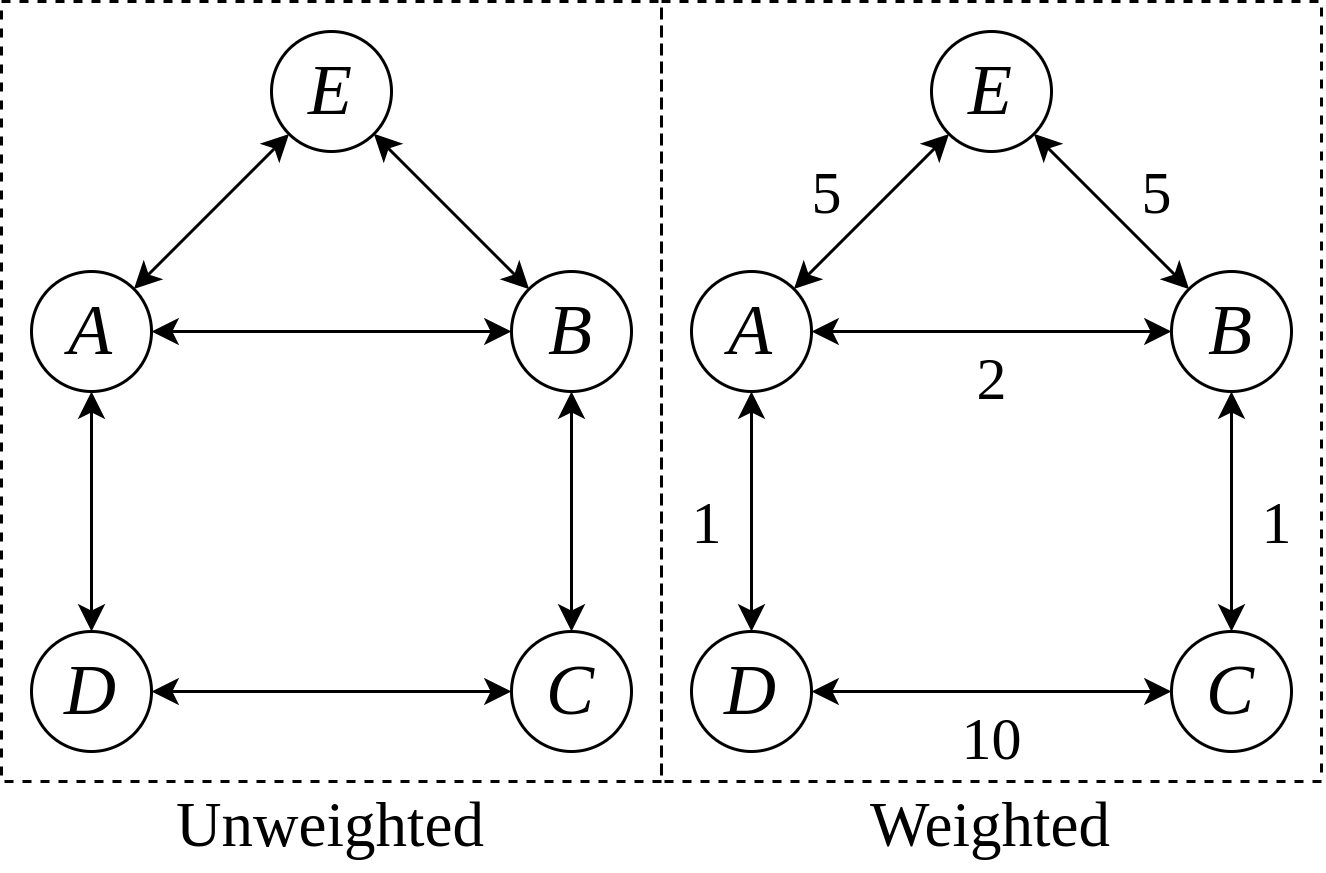
\includegraphics[width = .5\linewidth]{figs/simple_graph.png}
	\caption{Simple example undirected graph unweighted and weighted isomorphs (from \cite{Stephenson_1989})}
	\label{fig:simple_graph}
\end{figure}

From Figure \ref{fig:simple_graph} it is apparent that $A$ and $B$ are more central than the other nodes. Graphs, however, need not have a geometric center nor any plainly obvious 2-D geometry. Take, for example, a network of communications satellites in low Earth orbit. Although the state of the network could, at any point, be projected onto a 2-D surface it would be arbitrary where the corners of the map should be located. In 3-D space all satellites would be approximately the same distance from the geometric center, the center of the Earth, a location where there will be no proximate satellites. Centrality, thus, must have a more abstract definition. There are four commonly used metrics for centrality, degree centrality, closeness centrality, betweenness centrality, and information centrality. These will be defined in the below subsections.

\subsection{Degree Centrality}

A computationally simple way to compute adjacency-focused centrality is degree centrality. Degree centrality is defined as

\begin{equation}
	\Omega_d(v) = \frac{\eta(v)}{n - 1}
\end{equation}

where $\eta(v)$ is a function returning a value computed from the adjacency of node $v$. Degree is the number of adjacent nodes adjacent to a given node. A cell tower has high degree centrality as part of the cellular communications network.

\subsection{Closeness Centrality}

For a graph $G$, the sets of shortest paths from each node $v$ to all other nodes $R_{v,U}$ and vice versa $R_{U,v}$ are known. Closeness centrality is defined as

\begin{equation}
	\Omega_c(v) = \frac{n - 1}{\sum_{u \in U} \eta(v, u)}
\end{equation}

where $n$ is the cardinality of $V$ and $\eta(v, u)$ is the cost of the shortest path from $v$ to $u$. Closeness centrality reflects how close a given node is to those nodes reachable from it via shortest paths. St. Louis has high closeness centrality as part of the US freeway system.

\subsection{Betweenness Centrality}

For a graph $G$, the sets of shortest paths from each node $v$ to all other nodes $R_{v,U}$ and vice versa $R_{U,v}$ are known. Betweenness centrality is defined as

\begin{equation}
	\Omega_b(v) = \sum_{o, d \in V}\frac{\sigma(o, d\ |\ v)}{\sigma(o, d)}\label{eq:betweenness_centrality}
\end{equation}

where $\sigma(o, d\ |\ v)$ is the weighted sum of the set of shortest paths between $o$ and $d$ which contain $v$ and $\sigma(o, d)$ is the weighted sum of the set of shortest paths between $o$ and $d$. Betweenness centrality reflects the relative volume of use for a node in a graph (and may also be computed for edges). The Denver airport has high betweenness centrality as part of the US domestic aviation network.

\subsection{Information Centrality}

Conceptually the information content of a node on a graph is the path information gained after leaving that node. There may be many paths on a graph which pass through a given node and thus an expectation must be computed. The following derivation is based on \cite{Stephenson_1989} which is the original publication on information centrality.

For each O/D pair in $o,d \in V$ there is a set of paths $P_{od} = \{P_{od}(1),P_{od}(2), \dots, P_{od}(n_{od})\}$ with associated costs $C_{od}$. Picking $o=A$ and $d=B$ from the graph in Figure \ref{fig:simple_graph}, $P_{AB}$ contains $P_{AB}(1) = A - B$, $P_{AB}(2) = A - E - B$, and $P_{AB}(3) = A - D - C - B$. The costs of the paths will be $C_{AB}(1) = 1$, $C_{AB}(2) = 2$, and $C_{AB}(3) = 3$ for the unweighted graph and $C_{AB}(1) = 2$, $C_{AB}(2) = 10$, and $C_{AB}(3) = 12$ for the weighted graph. Under the assumption that lower-cost paths are more likely to be taken and knowing that information is inversely proportional to probability it should be apparent that the information content of the indirect paths is greater than that of the direct path. It should also be apparent that the edge weights increase the information disparity. Consider $I_{od}(i) = C_{od}(i)^{-1}$ as an analogue for information content (this is used rather than \eqref{eq:information_content} for computational simplicity). Entropy for node $o$ with respect to node $d$ can thus be computed as

\begin{equation}
	S_{od} = \sum_{i = 1}^{n_{od}}W_{od}(i)C_{od}(i)
\end{equation}

where

\begin{equation}
	W_{od}(i) = \frac{I_{od}(i)}{\sum_{i = 1}^{n_{od}} I_{od}(i)}
\end{equation}

Generalizing path entropy to node entropy means considering how node $o$ interacts with all possible O/D pairs which. For the sake of computational efficiency, this generalization can be formulated into a matrix-operations based process as in \cite{Stephenson_1989}. Information centrality for the nodes in $G = \{V, E\}$ is based on the inverse incidence matrix $B$ whose elements are

\begin{align}
	b_{ij} = \begin{cases}
		1 & (i, j) \not\in E \\
		1 - \eta(i, j) & otherwise
	\end{cases}\\
	b_{ii} = 1 + \sum_{(i, j) \in E_i} \eta(i, j)
\end{align}

where $\eta(i, j)$ is a function returning edge costs. The diagonal elements of $B$ are the degrees of $V$ plus self-connection and the non-diagonal elements are 1 if no direct connection exists and less than 1 where one does exist. Rows and columns of $B$ all have the same sum if $G$ is reciprocal. The information for each node can be computed form the incidence matrix $C = D^{-1}$ as

\begin{equation}
	\Omega_i(v) = \frac{n}{nc_{vv} + \sum_{u = 1}^{n} c_{uu} - 2 \sum_{u = 1}^{n}c_{vu}}\label{eq:information_centrality}
\end{equation}

Information centrality for a node should be interpreted as being, roughly, the degree to which that node is determinative of future nodes on a path between an unknown origin and destination. A node with high information content is a node which both appears on many lowest-cost paths and one which, generally, limits the set of paths after it. As an example, the phrase "medium-rare" may be preceded by many words but will usually be followed by a type of red meat. Information centrality should be thought of as the opposite of network entropy.

\subsection{Comparison}

The methods of computing centrality are compared for the simple graph shown in Figure \ref{fig:simple_graph}.

\begin{table}[H]
	\centering
	\caption{Centrality for simple undirected and unweighted example graph}
	\label{tab:unweighted_centrality}
	\begin{tabular}{|C{.2\linewidth}|C{.2\linewidth}|C{.2\linewidth}|C{.2\linewidth}|C{.2\linewidth}|}
		\hline Node & Degree Centrality & Betweenness Centrality & Closeness Centrality & Information Centrality \\
		\hline A & 0.75 & 0.25 & 0.8 & 0.355 \\
		\hline B & 0.75 & 0.25 & 0.8 & 0.355 \\
		\hline C & 0.5 & 0.083 & 0.667 & 0.282 \\
		\hline D & 0.5 & 0.083 & 0.667 & 0.282 \\
		\hline E & 0.5 & 0 & 0.667 & 0.275 \\
		\hline
	\end{tabular}
\end{table}

\begin{table}[H]
	\centering
	\caption{Centrality for simple undirected and weighted example graph}
	\label{tab:weighted_centrality}
	\begin{tabular}{|C{.2\linewidth}|C{.2\linewidth}|C{.2\linewidth}|C{.2\linewidth}|C{.2\linewidth}|}
		\hline Node & Degree Centrality & Betweenness Centrality & Closeness Centrality & Information Centrality \\
		\hline A & 0.75 & 0.5 & 0.364 & 0.667 \\
		\hline B & 0.75 & 0.5 & 0.364 & 0.667 \\
		\hline C & 0.5 & 0 & 0.286 & 0.535 \\
		\hline D & 0.5 & 0 & 0.286 & 0.535 \\
		\hline E & 0.5 & 0 & 0.182 & 0.646 \\
		\hline
	\end{tabular}
\end{table}

Concerning the isomorphs in Figure \ref{fig:simple_graph}, intuition would say that nodes $A$ and $B$ are most central and this is supported by all centrality measures presented. The principle effects of considering edge weights are that the shortest paths between $C$ and $D$ no longer utilize $(C, D)$, all shortest paths include $A$ or $B$, and 3 include $(A, B)$. The differences are not attested to by degree centrality which is identical among isomorphs. The increased reliance of the network on $A$ and $B$ is reflected in the remaining centrality metrics. The lower diversity of paths for the weighted graph is reflected in lower nodal information content.



\section{Topographical Entropy Maximization}

Entropy maximization is any system parameter optimization which has the goal of maximizing system entropy. As an example, the entropy of a series of coin flips is maximized if the coin is "fair" with $p(h) = 1 - p(t) = 0.5$. For a graph, entropy is maximized where information centrality is minimized. As shown in Tables \ref{tab:unweighted_centrality} and \ref{tab:weighted_centrality}, changing the edge weights of Figure \ref{fig:simple_graph} results in different levels of entropy. In theory, a graph may have no identifiable most-central node. The most obvious form of such a graph would be one where only the "outer" links are present (a triangle for example). The end result would be equal information centrality for each node. Note, however, that the nodes of a triangle would have higher information centrality than those of a square etc. due to the greater optionality of the higher-sided shapes.

Entropy maximization can be readily applied to transportation planning. Take, for example, the road network diagrammed in Figure \ref{fig:divided_network}.

\begin{figure}[H]
	\centering
	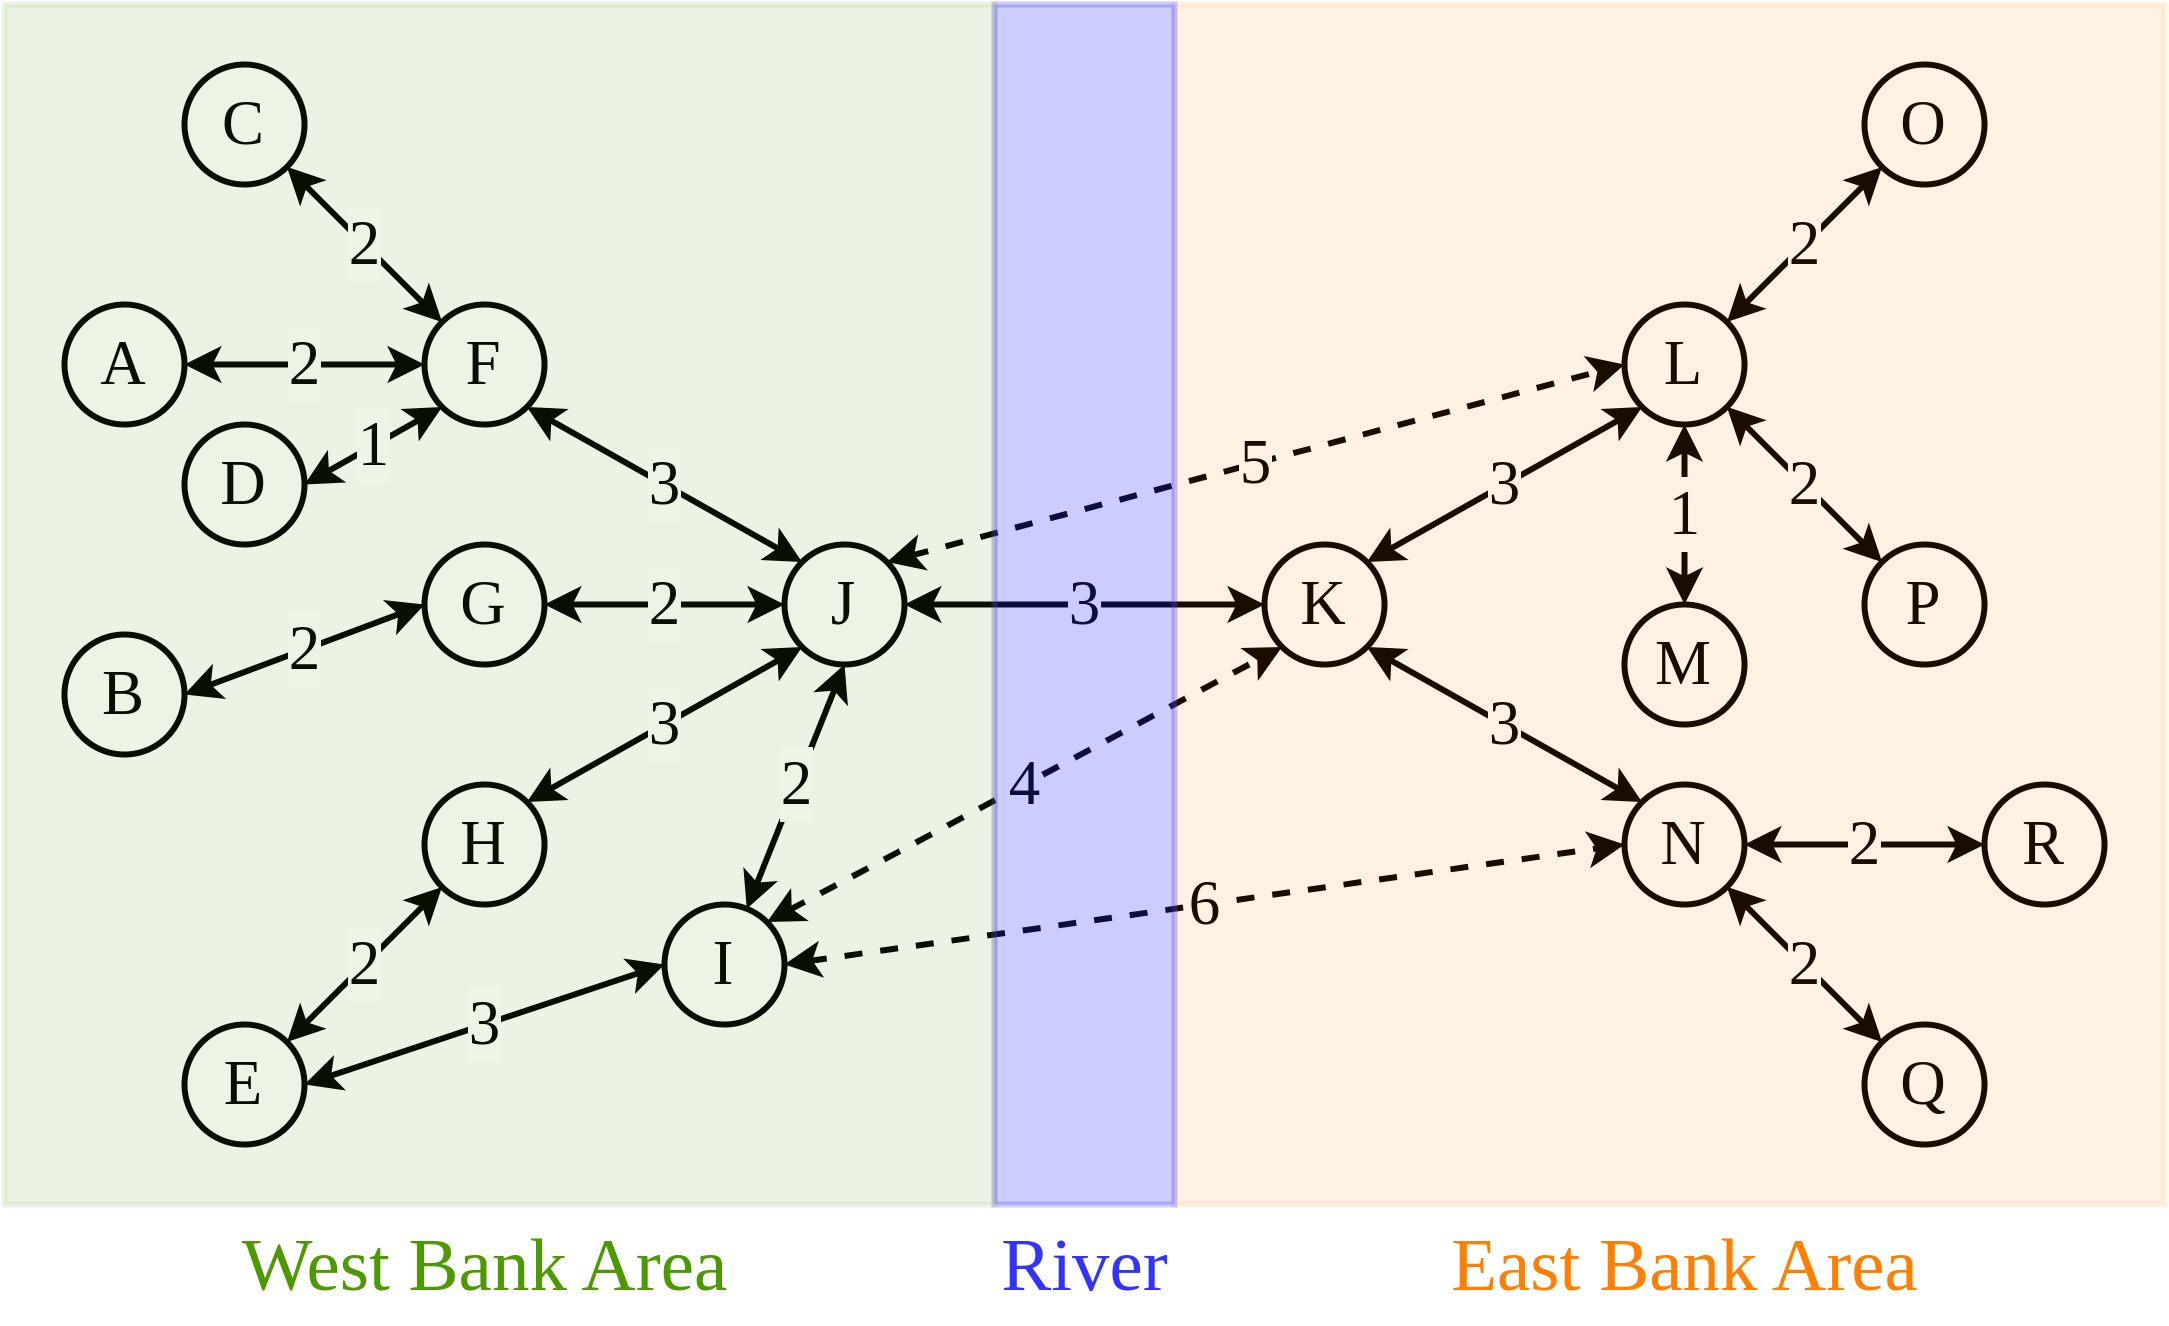
\includegraphics[width = .8\linewidth]{figs/divided_network.png}
	\caption{Example road network for city divided by a river. The solid links are present and dashed links are proposed additional links.}
	\label{fig:divided_network}
\end{figure}

The example city is, roughly, bifurcated by a river and the east and west bank areas are connected by a solitary bridge (J, K). It is evident that this bridge will feature in all shortest paths for O/D pairs on opposite sides of the river and is, thus both congested and a single point of failure for the network. Planners, thus, want to add at least one more bridge and have proposed the dashed links (I, N), (I, K), and (J, L). Information centrality for the network subject to the proposed additional brides is listed in Table \ref{tab:bridge_information_centrality}.

\begin{table}[H]
	\centering
	\caption{Information centrality for example road network subject to bridge additions}
	\label{tab:bridge_information_centrality}
	\begin{tabular}{|C{.2\linewidth}|C{.2\linewidth}|C{.2\linewidth}|C{.2\linewidth}|C{.2\linewidth}|}
		\hline Node & Baseline & (I, N) & (I, K) & (J, L) \\
		\hline A & 0.040 & 0.043 & 0.042 & 0.044 \\
		\hline F & 0.058 & 0.065 & 0.062 & 0.068 \\
		\hline B & 0.035 & 0.037 & 0.036 & 0.038 \\
		\hline G & 0.048 & 0.052 & 0.051 & 0.055 \\
		\hline C & 0.040 & 0.043 & 0.042 & 0.044 \\
		\hline D & 0.030 & 0.032 & 0.031 & 0.033 \\
		\hline E & 0.051 & 0.064 & 0.061 & 0.058 \\
		\hline H & 0.057 & 0.066 & 0.063 & 0.067 \\
		\hline I & 0.053 & 0.075 & 0.073 & 0.062 \\
		\hline J & 0.072 & 0.083 & 0.079 & 0.088 \\
		\hline K & 0.069 & 0.078 & 0.079 & 0.079 \\
		\hline L & 0.056 & 0.062 & 0.063 & 0.082 \\
		\hline N & 0.054 & 0.075 & 0.060 & 0.060 \\
		\hline O & 0.039 & 0.042 & 0.042 & 0.049 \\
		\hline P & 0.039 & 0.042 & 0.042 & 0.049 \\
		\hline M & 0.030 & 0.031 & 0.031 & 0.035 \\
		\hline R & 0.038 & 0.047 & 0.041 & 0.040 \\
		\hline Q & 0.038 & 0.047 & 0.041 & 0.040 \\
		\hline \textbf{Sum} & \textbf{0.844} & \textbf{0.981} & \textbf{0.937} & \textbf{0.992} \\
		\hline
	\end{tabular}
\end{table}

Besides the obvious conclusion that adding a second bridge increases entropy, a few interesting observations can be made. First, that the (J, L) bridge increases entropy more than the (I, N) bridge both for the network in general and for node J in particular. Second that bridge (I, N) similarly outperforms bridge (I, K). Both can be explained by looking at the structure of the network in the east bank area. Because node I is fairly isolated compared to node J, extra bridges from node I are less impactful than those from node J. The same can be said for nodes N and K. Thus, as presently structured (trees connected at the tip or the "traffic broccoli") adding bridges from one of the central nodes is most effective.

\section{\gls{evse} Entropy Maximization}

\gls{evse} location optimization is a topic which has produced, continues to produce, and will continue to produce ludicrous volumes of research very little of which informs deployment in any real way. This situation is the result of the fact that \gls{evse} infrastructure is insufficient in many ways and is perceived to serve as a impediment to \gls{pev} sales growth meaning that the large body of optimization and data analysis focused researchers are able to fund projects and publish papers related to the topic. In the most general sense, optimization of \gls{evse} locations is not an especially unique problem and most seek to optimize the allocation of scarce development resources to minimize a given cost function. A common theme of these papers is the goal of optimizing efficiency in metrics which are either business or consumer oriented. Robustness is often treated as a constraint if considered at all. This line of thinking has led to large concentrations of \gls{evse} in those areas most dense with \gls{pev} ownership and a number of subsidized charging stations located at arbitrary intervals along major transportation corridors. Evenly spaced chargers along corridors is not necessarily a bad solution but it is an arbitrary one.

Consider, instead, how redundancy might be computed from and informational perspective. As a driver embarks on a long trip (one that requires charging), the driver will have a charging window. The charging window starts at a distance where a substantial portion of the vehicle's range is used and will end when the driver is close enough to the destination that additional range is not required. For example, if a car has 300 km of range and is undertaking a 400 km trip at least one charge is required. However there will be little region to charge in the first 100 km because doing so will mean having to charge twice. For the same reason the last 100 km is unlikely to see a charge event. Thus, the charging window for the trip is the 200 km in the middle. If chargers were evenly spaced in 50 km intervals along the driver's route then of the 7 chargers available the middle 5 would be viable options. Since the driver only needs to charge once there is real redundancy built in. At the beginning of the trip there are 5 shortest paths that the driver must choose between. If the driver passes the first middle charger without charging then the number of shortest paths goes from 5 to 4, if the driver charges at the first middle charger then the number of shortest paths goes from 5 to 1. In this scenario charging provides more information than not charging and this is not surprising, stopping to charge will be less common than passing a charger.

In the above example the trip origin and destination as well as the vehicle range are known allowing for the definition of a charging window. In practice, these quantities can only be imputed stochastically. The basic principle, however, can be generalized:

\begin{lemma}[Charger-Charger Edge Energy Cost Upper Limit]
	Under normal circumstances, vehicles will not travel from charger $u$ to charger $v$ if the edge energy cost $d(u, v)$ is greater than a given upper limit $L^U$ which is less than or equal to the vehicle's maximum energy storage capability.
\end{lemma}

\begin{corollary}
	Chargers $u$ and $v$ are incident if and only if $d(u, v) < L^U$.
\end{corollary}

\begin{lemma}[Charger-Charger Edge Energy Cost Lower Limit]
	Under normal circumstances, vehicles will not travel from charger $u$ to charger $v$ if the edge energy cost $d(u, v)$ is less than a given lower limit $L^L$ which is greater than or equal to the vehicle's minimum energy storage capability.
\end{lemma}

\begin{corollary}
	Chargers $u$ and $v$ are incident if and only if $d(u, v) > L^L$.
\end{corollary}

\begin{lemma}[Charger-Place Edge Energy Cost Upper Limit]
	Under normal circumstances, vehicles will not travel from charger $u$ to place $v$ if the edge energy cost $d(u, v)$ is greater than a given upper limit $L^L$ which is less than or equal to the vehicle's minimum energy storage capability. The same holds for place-charger edges.
\end{lemma}

\begin{corollary}
	Charger $u$ and place $v$ are incident if and only if $d(u, v) < L^U$.
\end{corollary}

\begin{lemma}[Place-Place Edge Energy Cost Upper Limit]
	Under normal circumstances, vehicles will not travel from place $u$ to place $v$ if the edge energy cost $d(u, v)$ is greater than a given upper limit $L^L$ which is less than or equal to the vehicle's minimum energy storage capability.
\end{lemma}

\begin{corollary}
	Place $u$ and place $v$ are incident if and only if $d(u, v) < L^U$.
\end{corollary}

In other words, chargers relationships with each other are determined by distance. If two chargers are very far apart then it is unlikely that a car will travel from one to the other without having to charge at a third location. If two chargers are close together a vehicle may use either on a given trip but is unlikely to use both. The constants $L^L$ and $L^U$ define the span of incidence. Chargers themselves serve to allow for trips between places and, thus, will only be visited for the purposes of charging. Places can be visited at any \gls{soc} so there is no minimum edge cost for incidence if the edge connects at least one place node.
	

\printbibliography

\end{document}